\documentclass[11pt,a4paper]{article}

% ------------------------------------------------------------------ pacotes
\usepackage[utf8]{inputenc}
\usepackage[T1]{fontenc}
\usepackage[brazil]{babel}
\usepackage{lmodern}
\usepackage{microtype}
\usepackage[margin=2cm]{geometry}
\usepackage{amsmath,amssymb,amsthm}
\usepackage{graphicx}
\usepackage{booktabs}
\usepackage{array}
\usepackage{float}
\usepackage{caption}
\usepackage{xcolor}
\usepackage{listings}
\usepackage{algorithm}
\usepackage{algpseudocode}
\usepackage{enumitem}
\usepackage[hidelinks]{hyperref}

\newcommand{\kmin}{11}
\newcommand{\qtdcaminhos}{4}
\newcommand{\sequenciagraus}{(6, 5, 5, 5, 5, 4, 4, 3, 3, 3, 3, 3, 3, 3, 3, 3, 3, 2, 2, 2, 2, 2, 2, 2, 2)}
\newcommand{\grauminimo}{2}
\newcommand{\graumaximo}{6}
\newcommand{\somagraus}{80}
\newcommand{\impares}{14}


% ------------------------------------------------------------------ ambientes
\theoremstyle{definition}
\newtheorem{definicao}{Definição}[section]
\newtheorem{observacao}[definicao]{Observação}
\theoremstyle{plain}
\newtheorem{teorema}[definicao]{Teorema}
\newtheorem{proposicao}[definicao]{Proposição}
\newtheorem{lema}[definicao]{Lema}
\newtheorem{corolario}[definicao]{Corolário}
\renewcommand{\qedsymbol}{C.Q.D.}

\floatname{algorithm}{Algoritmo}
\renewcommand{\algorithmicrequire}{\textbf{Entrada:}}
\renewcommand{\algorithmicensure}{\textbf{Saída:}}

\newcommand{\repo}{\url{https://github.com/Mazzoni-mat-ap/Codigos_discreta}}
\newcommand{\dE}{d_{E}}

% ------------------------------------------------------------------ código
\definecolor{fundo}{HTML}{F6F8FA}
\definecolor{comentario}{HTML}{6A737D}
\definecolor{palavra}{HTML}{1D4ED8}
\definecolor{texto}{HTML}{0F766E}
\lstset{
  language=Python,
  basicstyle=\ttfamily\footnotesize,
  keywordstyle=\color{palavra}\bfseries,
  commentstyle=\color{comentario}\itshape,
  stringstyle=\color{texto},
  backgroundcolor=\color{fundo},
  numbers=left, numberstyle=\tiny\color{comentario}, numbersep=6pt,
  frame=single, rulecolor=\color{black!15},
  breaklines=true, showstringspaces=false, tabsize=4,
  columns=fullflexible, keepspaces=true,
  extendedchars=true,
  literate=
    {á}{{\'a}}1 {â}{{\^a}}1 {ã}{{\~a}}1 {à}{{\`a}}1
    {é}{{\'e}}1 {ê}{{\^e}}1 {í}{{\'i}}1
    {ó}{{\'o}}1 {ô}{{\^o}}1 {õ}{{\~o}}1 {ú}{{\'u}}1
    {ç}{{\c{c}}}1 {Ú}{{\'U}}1 {É}{{\'E}}1 {Ã}{{\~A}}1
}

% ------------------------------------------------------------------ documento
\begin{document}

\begin{titlepage}
  \centering
  {\large FGV EMAp --- Escola de Matemática Aplicada\par}
  {\large Matemática Discreta\par}
  \vspace{4cm}
  {\LARGE\bfseries Caminhos Mínimos com Matemática Discreta\par}
  \vspace{0.4cm}
  {\Large Otimização de rotas de fuga por meio de algoritmos aplicados em Teoria dos Grafos\par}
  \vspace{3cm}
  {\large
    Frederico Taveira Martins de Souza\\[2pt]
    Ian Luca Marinho Aguiar\\[2pt]
    João Vitor Neves Mazzoni\\[2pt]
    Marcelo Maiato Neves\par}
  \vfill
  {\large Rio de Janeiro, novembro de 2026\par}
\end{titlepage}

\begin{abstract}
Situações de evacuação, como uma enchente em uma cidade ou um alarme em um
laboratório, têm sempre a mesma estrutura: salas ligados por passagens, um
ponto de partida, uma saída e um tempo limite. A Teoria dos Grafos é a forma perfeita de lidar com este problema, pois transforma a pergunta ``por onde fugir?''
em perguntas sobre caminhos, distâncias e conexidade, tais que
existem algoritmos cuja correção pode ser demonstrada. O objetivo deste trabalho é
modelar e demonstrar, a partir da Teoria dos Grafos, formas otimizadas de
encontrar rotas de fuga em contextos distintos. Escolhemos como escopo um
\emph{escape room}, a \emph{Fuga do Laboratório}: um ambiente controlado, com
regras explícitas, em que o problema pode ser enunciado e verificado por
completo. Resolvido o problema da travessia entre as salas de um \textit{escape room}, a
mesma lógica de resolução se aplica a contextos reais, como a evacuação de
regiões atingidas por enchentes. A metodologia consiste em modelar o ambiente como um grafo
com pesos, em que salas são vértices, portas são arestas e os pesos são os tempos
de travessia; reunir e demonstrar as definições e propriedades necessárias;
contrapor dois critérios de otimização de rotas, o menor número de portas, obtido
pela busca em largura, e o menor tempo, obtido pelo Algoritmo de Dijkstra; e
caracterizar as salas cuja obstrução impede a fuga. Todos os algoritmos foram
implementados em Python e reunidos em um simulador interativo, no qual também
aplicamos o modelo a um cenário de enchente. O relatório apresenta as
definições e propriedades utilizadas, os algoritmos com suas demonstrações de
correção, os exemplos simulados e, na conclusão, os resultados obtidos. O código
e o simulador estão disponíveis em \repo.
\end{abstract}

\tableofcontents
\newpage

\section{Introdução}

Planejar uma rota de fuga é decidir, entre muitas sequências possíveis de
ambientes, qual leva da posição atual até a saída da melhor maneira. A Teoria dos
Grafos oferece exatamente as ferramentas para isso: assim como no problema das
pontes de Königsberg, partimos de uma situação concreta, construímos um modelo
matemático e traduzimos a pergunta original para o modelo, onde ela pode ser
respondida com rigor.

O objetivo deste trabalho é modelar e demonstrar, a partir da Teoria dos Grafos,
formas otimizadas de encontrar rotas de fuga. Escolhemos um escape room porque ele
reúne, em escala controlada, todos os elementos de uma evacuação real (salas,
passagens, tempo limite e obstáculos) e permite verificar cada resposta. Uma vez
resolvido o problema da travessia entre as salas, a mesma lógica se aplica a
outros contextos, como mostramos ao final com um cenário de enchente.

\paragraph{A história.} Durante uma visita ao laboratório da professora, um
experimento dá errado: o alarme toca, as portas se trancam e, em 40 minutos, o
prédio será selado. A professora está presa na sala de controle e avisa pelo
rádio que, para chegar até ela e sair, é preciso passar pela Portaria (onde está o
crachá que destrava os laboratórios), pela Sala das máscaras (os laboratórios
estão com fumaça), pela Sala de limpeza (quem sai da fumaça precisa se limpar),
pela Sala das câmeras (onde se descobre a senha do depósito) e, por fim, pela
própria Sala de controle, que desliga o alarme e abre a saída.

\paragraph{Desafio:} \emph{é possível sair da entrada e chegar à saída em no
máximo 40 minutos? Se sim, por onde?}

\paragraph{Modelo.} Cada sala é um vértice e cada porta é uma aresta; o peso de
cada aresta é o tempo, em minutos, para atravessar o corredor correspondente
(Figura~\ref{fig:mapa} e Tabela~\ref{tab:nomes}). O grafo obtido é definido
formalmente na Definição~\ref{def:escape}, e o desafio passa a ser:

\paragraph{Desafio no modelo:} \emph{a distância entre a entrada e a saída é
menor ou igual a 40?} (Definições~\ref{def:distancia} e~\ref{def:fuga}).

\begin{figure}[H]
  \centering
  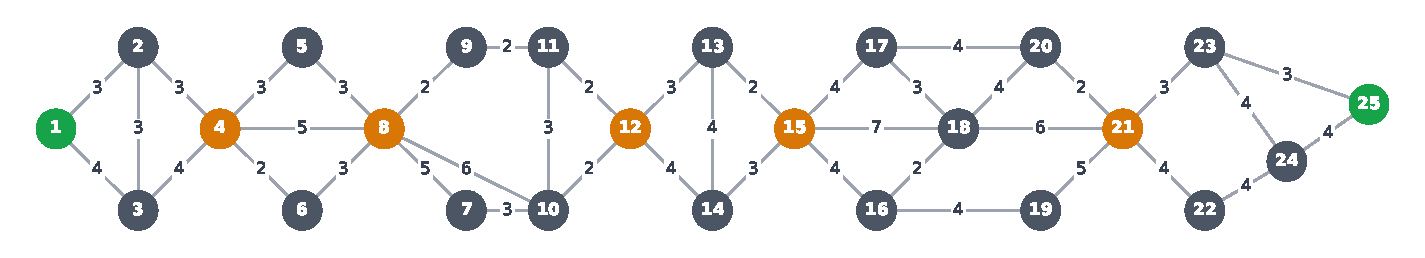
\includegraphics[width=\textwidth]{figuras/mapa.pdf}
  \caption{O grafo do escape room. Verde: entrada ($v_1$) e saída ($v_{25}$);
  laranja: as cinco salas obrigatórias da história. O número em cada aresta é o
  seu peso, em minutos.}
  \label{fig:mapa}
\end{figure}

\begin{table}[H]
  \centering
  \caption{Nome de cada sala.}
  \label{tab:nomes}
  \small
  \begin{tabular}{rl|rl|rl}
\toprule
$v_{1}$ & Entrada & $v_{2}$ & Recepção & $v_{3}$ & Sala de espera \\
$v_{4}$ & Portaria & $v_{5}$ & Vestiário & $v_{6}$ & Almoxarifado \\
$v_{7}$ & Laboratório de química & $v_{8}$ & Sala das máscaras & $v_{9}$ & Laboratório de biologia \\
$v_{10}$ & Laboratório de física & $v_{11}$ & Laboratório de microscopia & $v_{12}$ & Sala de limpeza \\
$v_{13}$ & Arquivo de documentos & $v_{14}$ & Arquivo de amostras & $v_{15}$ & Sala das câmeras \\
$v_{16}$ & Depósito de reagentes & $v_{17}$ & Depósito de equipamentos & $v_{18}$ & Depósito central \\
$v_{19}$ & Câmara fria & $v_{20}$ & Depósito de vidraria & $v_{21}$ & Sala de controle \\
$v_{22}$ & Corredor de serviço & $v_{23}$ & Hall de saída & $v_{24}$ & Sala de segurança \\
$v_{25}$ & Saída &  &  &  &  \\
\bottomrule
\end{tabular}

\end{table}

\paragraph{Organização.} A Seção~\ref{sec:definicoes} reúne todas as definições
utilizadas, separando as definições gerais da Teoria dos Grafos das definições
próprias deste trabalho, junto com as propriedades que delas decorrem. A
Seção~\ref{sec:resultados} apresenta a busca em largura e o Algoritmo de Dijkstra,
demonstra a correção de cada um e os contrapõe no grafo do escape room. A
Seção~\ref{sec:exemplos} traz os cenários simulados, incluindo um cenário de
enchente, e a Seção~\ref{sec:conclusao} resume os resultados.

\section{Definições básicas e propriedades}\label{sec:definicoes}

Os algoritmos usados neste trabalho só garantem rotas ótimas porque se apoiam em
propriedades que podem ser demonstradas. Por isso, reunimos nesta seção todas as
definições utilizadas no relatório, numeradas para serem citadas adiante, e
demonstramos cada propriedade de que precisamos. Separamos as definições gerais,
que são convenções da Teoria dos Grafos e seguem as notas de aula~\cite{notas},
das definições próprias deste trabalho, criadas para modelar o problema da fuga.

\subsection{Definições gerais}

\begin{definicao}[Grafo]\label{def:grafo}
Um GRAFO $G$ é constituído por dois conjuntos $V$ e $E$, onde os elementos de $V$
são chamados de VÉRTICES e $E$ é um conjunto de pares não-ordenados de elementos
de $V$, chamados de ARESTAS. Escreve-se $G=(V,E)$. Neste trabalho, todo grafo é
finito.
\end{definicao}

\begin{definicao}[Adjacência e grafo simples]\label{def:simples}
Seja $G=(V,E)$ um grafo e $e = \{v_i, v_j\} \in E$. Diz-se que $v_i$ e $v_j$ são
ADJACENTES e que $e$ INCIDE em $v_i$ e $v_j$. Se $v_i = v_j$, a aresta $e$ é um
LAÇO. Um grafo é dito SIMPLES se não possui laços nem arestas paralelas (arestas
distintas com os mesmos extremos).
\end{definicao}

\begin{definicao}[Vizinhança]\label{def:vizinhanca}
Dado $G=(V,E)$ e $v \in V$, a VIZINHANÇA de $v$ é o conjunto
$N(v) = \{u \in V : \{u,v\} \in E\}$ dos vértices adjacentes a $v$.
\end{definicao}

\begin{definicao}[Grafo com pesos]\label{def:pesos}
Um GRAFO COM PESOS é um grafo $G=(V,E)$ no qual cada aresta $e$ tem associado um
número real $w(e)$, chamado de PESO da aresta. Para $e = \{u,v\}$, escreve-se
também $w(u,v)$.
\end{definicao}

\begin{definicao}[Subgrafo e remoções]\label{def:subgrafo}
Dados $G=(V,E)$ e $G'=(V',E')$, diz-se que $G'$ é SUBGRAFO de $G$ se
$V' \subseteq V$, $E' \subseteq E$ e toda aresta de $E'$ tem seus extremos em
$V'$. Para $S \subseteq V$, $G \setminus S$ denota o subgrafo obtido removendo de
$G$ os vértices de $S$ e todas as arestas que incidem neles; para $e \in E$,
$G \setminus \{e\}$ denota o subgrafo obtido removendo apenas a aresta $e$.
\end{definicao}

\begin{definicao}[Caminho]\label{def:caminho}
Seja $G=(V,E)$ um grafo e sejam $v_0, v_n \in V$. Um CAMINHO de COMPRIMENTO $n$
de $v_0$ até $v_n$ é uma sequência alternando vértices e arestas, com $n+1$
vértices e $n$ arestas (permitindo repetições),
$P = (v_0, e_1, v_1, e_2, \dots, e_n, v_n)$, onde $e_i = \{v_{i-1}, v_i\}$ para
$i = 1, \dots, n$. Denotamos o comprimento por $\ell(P) = n$. Num grafo simples,
escreve-se só a sequência de vértices $(v_0, v_1, \dots, v_n)$. Um CAMINHO
SIMPLES é um caminho em que nenhum vértice aparece mais de uma vez.
\end{definicao}

\begin{definicao}[Comprimento com pesos]\label{def:compesos}
Em um grafo com pesos, o COMPRIMENTO COM PESOS de um caminho $P$ é a soma dos
pesos das suas arestas, $w(P) = \sum_{i=1}^{n} w(e_i)$.
\end{definicao}

\begin{definicao}[Conexidade]\label{def:conexo}
Um grafo $G=(V,E)$ é CONEXO se, para todo par $u, v \in V$, existe um caminho em
$G$ de $u$ a $v$. A COMPONENTE CONEXA de $G$ que contém $v$ é o subgrafo formado
pelos vértices alcançáveis a partir de $v$ por algum caminho de $G$ e por todas
as arestas de $G$ cujos extremos estão nesse conjunto.
\end{definicao}

\begin{definicao}[Distâncias]\label{def:distancia}
Sejam $u, v$ vértices de um grafo $G$. A DISTÂNCIA EM ARESTAS $\dE(u,v)$ é o menor
comprimento $\ell(P)$ entre os caminhos $P$ de $u$ a $v$. Se $G$ tem pesos
positivos, a DISTÂNCIA $d(u,v)$ é o menor comprimento com pesos $w(P)$ entre esses
caminhos. Se não existe caminho de $u$ a $v$, define-se
$\dE(u,v) = d(u,v) = +\infty$.
\end{definicao}

\begin{definicao}[Matriz de adjacência]\label{def:adjacencia}
Seja $G=(V,E)$ um grafo simples com $n = |V|$ vértices rotulados
$v_1, \dots, v_n$. A MATRIZ DE ADJACÊNCIA de $G$ é a matriz
$A = (a_{ij}) \in \mathbb{R}^{n\times n}$ com $a_{ij} = 1$ se
$\{v_i, v_j\} \in E$ e $a_{ij} = 0$ caso contrário. Como as arestas não têm
orientação e não há laços, $A$ é simétrica e $a_{ii} = 0$.
\end{definicao}

\subsection{Definições próprias do trabalho}

\begin{definicao}[Matriz de pesos]\label{def:matrizpesos}
Seja $G=(V,E)$ um grafo simples com pesos e vértices $v_1, \dots, v_n$. A MATRIZ
DE PESOS de $G$ é $W = (w_{ij})$, com $w_{ii} = 0$, $w_{ij} = w(v_i, v_j)$ se
$\{v_i, v_j\} \in E$ e $w_{ij} = \infty$ caso contrário. Ela é a forma como o
programa recebe um grafo, e $a_{ij} = 1$ se, e somente se, $i \ne j$ e
$w_{ij} < \infty$.
\end{definicao}

\begin{definicao}[Grafo do escape room]\label{def:escape}
É o grafo simples, conexo e com pesos positivos $G=(V,E)$ em que
$V = \{v_1, \dots, v_{25}\}$ são as salas, $E$ são as 40 portas e $w(e)$ é o tempo,
em minutos, de cada corredor, dados pela matriz de pesos do
Apêndice~\ref{ap:matrizes}. A entrada é $s = v_1$, a saída é $t = v_{25}$ e o tempo
limite é $T = 40$.
\end{definicao}

\begin{definicao}[Rota de fuga e condição de fuga]\label{def:fuga}
Uma ROTA DE FUGA é um caminho de $s$ a $t$. Seu NÚMERO DE PORTAS é o comprimento
$\ell(P)$ (Definição~\ref{def:caminho}) e seu TEMPO é o comprimento com pesos
$w(P)$ (Definição~\ref{def:compesos}). A FUGA É POSSÍVEL se existe uma rota de
fuga com tempo menor ou igual a $T$, isto é, se $d(s,t) \le T$.
\end{definicao}

\begin{definicao}[Bloqueios]\label{def:bloqueio}
BLOQUEAR uma sala $v$ é passar do grafo $G$ para $G \setminus \{v\}$; FECHAR uma
porta $e$ é passar para $G \setminus \{e\}$ (Definição~\ref{def:subgrafo}).
\end{definicao}

\begin{definicao}[Sala obrigatória]\label{def:obrigatoria}
Um vértice $v \notin \{s,t\}$ é uma SALA OBRIGATÓRIA se $s$ e $t$ estão em
componentes conexas diferentes de $G \setminus \{v\}$.
\end{definicao}

\subsection{Propriedades}

A primeira propriedade garante que as distâncias da Definição~\ref{def:distancia}
estão bem definidas: como um caminho pode repetir vértices, existem infinitos
caminhos entre dois vértices, e precisamos mostrar que o menor valor existe.

\begin{proposicao}\label{prop:simples}
Sejam $u, v$ vértices de um grafo $G$ com pesos positivos, ligados por algum
caminho. Então os mínimos que definem $\dE(u,v)$ e $d(u,v)$ existem e são
atingidos por caminhos simples.
\end{proposicao}

\begin{proof}
Seja $P$ um caminho de $u$ a $v$ em que algum vértice $x$ aparece duas vezes.
Retirando de $P$ o trecho entre as duas ocorrências de $x$, obtemos um caminho de
$u$ a $v$ com comprimento menor e, como os pesos são positivos, com comprimento
com pesos menor. Repetindo o procedimento, que termina porque o comprimento
diminui a cada passo, chegamos a um caminho simples $P'$ com
$\ell(P') \le \ell(P)$ e $w(P') \le w(P)$. Como $G$ é finito, há uma quantidade
finita de caminhos simples de $u$ a $v$, e o menor valor entre eles é menor ou
igual ao de qualquer caminho. Logo os mínimos existem e são atingidos por caminhos
simples.
\end{proof}

\begin{teorema}\label{teo:potencias}
Seja $A$ a matriz de adjacência de um grafo simples $G$
(Definição~\ref{def:adjacencia}). Então, para todo $k \in \mathbb{Z}_+$, a entrada
$ij$ da matriz $A^k$ é a quantidade de caminhos de $v_i$ a $v_j$ de comprimento $k$.
\end{teorema}

\begin{proof}
Por indução em $k$.

\emph{Caso base} ($k = 1$): $a_{ij} = 1$ se existe aresta entre $v_i$ e $v_j$ e
$0$ caso contrário, e os caminhos de comprimento 1 são exatamente as arestas.

\emph{Hipótese indutiva:} a tese vale para $k$.

\emph{Passo indutivo:} temos $(A^{k+1})_{ij} = \sum_{l=1}^{n} (A^k)_{il}\, a_{lj}$.
Pela hipótese, $(A^k)_{il}$ conta os caminhos de comprimento $k$ de $v_i$ a $v_l$,
e $a_{lj}$ vale 1 se $\{v_l, v_j\}$ é aresta e 0 caso contrário. Assim, cada
parcela conta os caminhos de comprimento $k+1$ de $v_i$ a $v_j$ cujo penúltimo
vértice é $v_l$, e a soma sobre $l$ conta todos eles.
\end{proof}

As duas últimas propriedades justificam o nome dado na
Definição~\ref{def:obrigatoria} e mostram por que essas salas são críticas.

\begin{proposicao}\label{prop:obrigatoria}
Seja $G$ conexo e $v \notin \{s,t\}$. Então $v$ aparece em toda rota de fuga se, e
somente se, $v$ é uma sala obrigatória.
\end{proposicao}

\begin{proof}
($\Leftarrow$) Se alguma rota de fuga não passasse por $v$, ela também seria um
caminho em $G \setminus \{v\}$, e $s$ e $t$ estariam na mesma componente conexa de
$G \setminus \{v\}$, contradição.

($\Rightarrow$) Se $s$ e $t$ estivessem na mesma componente conexa de
$G \setminus \{v\}$, existiria nesse grafo um caminho de $s$ a $t$. Esse caminho
também está em $G$ e não passa por $v$, contradição.
\end{proof}

\begin{corolario}\label{cor:bloqueio}
Se $v$ é uma sala obrigatória, então em $G \setminus \{v\}$ vale
$d(s,t) = +\infty$. Em particular, bloquear $v$ torna a fuga impossível para
qualquer tempo limite $T$.
\end{corolario}

\begin{proof}
Pela Definição~\ref{def:obrigatoria}, não existe caminho de $s$ a $t$ em
$G \setminus \{v\}$; pela Definição~\ref{def:distancia}, $d(s,t) = +\infty > T$.
\end{proof}
\section{Resultados principais}\label{sec:resultados}

Nesta seção apresentamos os dois algoritmos que contrapomos para encontrar rotas
de fuga, demonstramos que cada um encontra a rota ótima segundo o seu critério e
aplicamos ambos ao grafo do escape room (Definição~\ref{def:escape}).

\subsection{Menos portas: busca em largura}

A busca em largura (BFS) explora o grafo em camadas: primeiro os vizinhos da
origem, depois os vizinhos dos vizinhos, e assim por diante. Ela ignora os pesos
e, como veremos, encontra a rota com o menor número de portas. Em aula, a mesma
busca foi apresentada como forma de construir uma árvore geradora de um grafo
conexo; aqui usamos os níveis dessa construção para medir distâncias em arestas.

\begin{algorithm}[H]
\caption{Busca em largura de $a$ até $z$}\label{alg:bfs}
\begin{algorithmic}[1]
\Require grafo $G=(V,E)$, vértices $a$ e $z$
\Ensure caminho de $a$ até $z$ com o menor número de arestas
\State marque $a$ como visitado; $\mathrm{nivel}(a) \gets 0$; $F \gets (a)$ \Comment{fila}
\While{$F$ não está vazia}
  \State retire o primeiro vértice $u$ de $F$
  \If{$u = z$} \Return o caminho de $a$ até $z$ refeito pelos pais \EndIf
  \For{cada $v \in N(u)$ ainda não visitado}
    \State marque $v$; $\mathrm{pai}(v) \gets u$; $\mathrm{nivel}(v) \gets \mathrm{nivel}(u)+1$; coloque $v$ no fim de $F$
  \EndFor
\EndWhile
\State \Return ``não existe caminho''
\end{algorithmic}
\end{algorithm}

\begin{lema}\label{lem:fila}
Em qualquer momento da execução, se $F = (u_1, \dots, u_r)$, então
$\mathrm{nivel}(u_1) \le \dots \le \mathrm{nivel}(u_r) \le \mathrm{nivel}(u_1) + 1$.
Em particular, os vértices saem da fila em ordem não decrescente de nível.
\end{lema}

\begin{proof}
No início, $F = (a)$ e a afirmação vale. Retirar o primeiro elemento preserva a
propriedade. Quando $u$ é retirado, a nova fila começa com um vértice de nível
pelo menos $\mathrm{nivel}(u)$ e termina com vértices de nível no máximo
$\mathrm{nivel}(u)+1$; os vértices inseridos em seguida têm nível exatamente
$\mathrm{nivel}(u)+1$, o que preserva as duas desigualdades.
\end{proof}

\begin{proposicao}\label{prop:bfs}
Executando o Algoritmo~\ref{alg:bfs} sem a parada da linha 4, um vértice $v$ é
visitado se, e somente se, existe caminho de $a$ a $v$; e, nesse caso,
$\mathrm{nivel}(v) = \dE(a,v)$ (Definição~\ref{def:distancia}). Em particular, o
caminho devolvido na linha 4 é uma rota com o menor número de arestas.
\end{proposicao}

\begin{proof}
Seguindo os pais a partir de um vértice visitado $v$, obtemos um caminho de $a$ a
$v$ com $\mathrm{nivel}(v)$ arestas; logo todo vértice visitado é alcançável e
$\mathrm{nivel}(v) \ge \dE(a,v)$. Reciprocamente, se $(a = x_0, \dots, x_k = v)$
é um caminho e $x_i$ fosse o primeiro vértice não visitado, então $x_{i-1}$ foi
visitado, entrou na fila e foi retirado dela, momento em que $x_i$ teria sido
visitado, contradição.

Suponha agora, por contradição, que existe $v$ com
$\mathrm{nivel}(v) > \dE(a,v)$, e escolha o de menor $\dE(a,v) = k$. Seja $u$ o
vértice anterior a $v$ em um caminho com $k$ arestas; então $\dE(a,u) = k-1$ e,
pela escolha de $v$, $\mathrm{nivel}(u) = k-1$. Quando $u$ é retirado da fila, ou
$v$ ainda não foi visitado, e então recebe $\mathrm{nivel}(v) = k$; ou $v$ já
entrou na fila antes, e pelo Lema~\ref{lem:fila} tem
$\mathrm{nivel}(v) \le \mathrm{nivel}(u) + 1 = k$. Nos dois casos,
$\mathrm{nivel}(v) \le k$, contradição.
\end{proof}

Como cada vértice entra na fila no máximo uma vez e cada aresta é examinada duas
vezes, a busca em largura faz $O(|V| + |E|)$ operações.

\subsection{Menor tempo: Algoritmo de Dijkstra}

Para levar em conta os pesos, usamos o Algoritmo de Dijkstra~\cite{dijkstra}, como
visto em aula. Seja $G=(V,E)$ um grafo com pesos positivos $w(u,v) > 0$. Cada
vértice $x$ recebe um RÓTULO $L(x)$, atualizado ao longo das iterações, e $T$
denota o conjunto dos vértices ainda não visitados.

\begin{algorithm}[H]
\caption{Dijkstra de $a$ até $z$}\label{alg:dijkstra}
\begin{algorithmic}[1]
\Require grafo $G=(V,E)$ com pesos positivos, vértices $a$ e $z$
\Ensure $L(z) = d(a,z)$ e um caminho de $a$ até $z$ com comprimento com pesos $L(z)$
\State $L(a) \gets 0$; $L(x) \gets +\infty$ para todo $x \ne a$; $T \gets V$
\While{$T \ne \emptyset$}
  \State escolha $v \in T$ com $L(v)$ mínimo
  \If{$L(v) = +\infty$} \textbf{pare} \Comment{os vértices restantes são inalcançáveis}
  \EndIf
  \State $T \gets T \setminus \{v\}$
  \For{cada $x \in N(v) \cap T$}
    \If{$L(v) + w(v,x) < L(x)$}
      \State $L(x) \gets L(v) + w(v,x)$; $\mathrm{pai}(x) \gets v$
    \EndIf
  \EndFor
\EndWhile
\end{algorithmic}
\end{algorithm}

\begin{teorema}\label{teo:dijkstra}
Seja $G=(V,E)$ um grafo com pesos positivos. Cada vez que o
Algoritmo~\ref{alg:dijkstra} retira um vértice $v$ de $T$ (linha 6), vale
$L(v) = d(a,v)$.
\end{teorema}

\begin{proof}
Por indução finita sobre o número de vértices já retirados de $T$.

\emph{B.I.:} na primeira iteração, o algoritmo retira $a$, com $L(a) = 0 = d(a,a)$.

\emph{H.I.:} suponha que, após $k$ iterações, o rótulo de cada um dos $k$ vértices
retirados de $T$ é igual à sua distância a partir de $a$.

\emph{P.I.:} na iteração $k+1$, seja $v$ o vértice retirado, ou seja,
$L(v) = \min\{L(u) : u \in T\}$. Todo rótulo finito é o comprimento com pesos do
caminho obtido seguindo os pais, logo $L(v) \ge d(a,v)$. Suponha, por contradição,
que existe um caminho $P$ de $a$ até $v$ com $w(P) < L(v)$. Seja $u$ o primeiro
vértice de $P$ que está em $T$ (pode ser o próprio $v$) e seja $x$ o vértice que
precede $u$ em $P$. Como $x$ já saiu de $T$, pela H.I. o trecho de $P$ até $x$ tem
comprimento com pesos pelo menos $L(x)$, e quando $x$ saiu de $T$ o rótulo de $u$
passou a ser no máximo $L(x) + w(x,u)$. Como os pesos são positivos e $u$ é
escolhido entre os de $T$,
\[
  w(P) \ <\ L(v) \ \le\ L(u) \ \le\ L(x) + w(x,u) \ \le\ w(\text{trecho de $P$ até $u$})
  \ \le\ w(P),
\]
o que é uma contradição. Logo $L(v) = d(a,v)$.
\end{proof}

\begin{corolario}\label{cor:dijkstra}
O algoritmo termina após no máximo $n = |V|$ iterações. Se $z$ é alcançável a
partir de $a$, então $L(z) = d(a,z)$ e o caminho de $a$ até $z$ obtido seguindo os
pais tem comprimento com pesos $d(a,z)$; caso contrário, $L(z) = +\infty$. Como
cada iteração procura o mínimo entre no máximo $n$ rótulos, a complexidade é
$O(n^2)$.
\end{corolario}

\begin{proof}
Cada iteração retira um vértice de $T$, logo há no máximo $n$ iterações. Se $z$ é
alcançável e o algoritmo parasse na linha 4 com $z \in T$, tomaríamos um caminho
de $a$ a $z$ e o seu primeiro vértice $u$ em $T$; o vértice anterior a $u$ já
saiu de $T$ com rótulo finito, logo $L(u) < +\infty$, contradizendo a parada.
Assim $z$ é retirado de $T$ e, pelo Teorema~\ref{teo:dijkstra}, $L(z) = d(a,z)$.
O caminho pelos pais tem comprimento com pesos $L(z)$, pois a linha 9 sempre faz
$L(x) = L(\mathrm{pai}(x)) + w(\mathrm{pai}(x), x)$. Se $z$ não é alcançável,
nenhum caminho pelos pais chega a $z$, e seu rótulo permanece $+\infty$.
\end{proof}

\begin{observacao}
A positividade dos pesos é usada na demonstração e é garantida pelo modelo
(Definição~\ref{def:escape}): atravessar um corredor sempre leva algum tempo.
\end{observacao}

\subsection{Contraposição dos dois critérios no escape room}

Aplicamos agora os dois algoritmos ao grafo da Definição~\ref{def:escape}, com
$a = s = v_1$ e $z = t = v_{25}$.

\paragraph{Menor tempo.} Pelo Teorema~\ref{teo:dijkstra}, o Algoritmo de Dijkstra
fornece $d(v_1, v_{25}) = 38$, com a rota
\[
  v_1 \to v_2 \to v_4 \to v_8 \to v_9 \to v_{11} \to v_{12} \to v_{13} \to v_{15}
  \to v_{17} \to v_{20} \to v_{21} \to v_{23} \to v_{25},
\]
de 13 portas. Como $38 \le 40$, pela Definição~\ref{def:fuga} a fuga é possível,
com folga de apenas 2 minutos.

\paragraph{Menos portas.} Pela Proposição~\ref{prop:bfs}, a busca em largura
fornece uma rota com $\dE(v_1, v_{25})$ portas. Mostramos a seguir, sem depender
do algoritmo, que esse número é \kmin{} e que nenhuma rota com \kmin{} portas
cabe no tempo limite.

\begin{proposicao}\label{prop:onze}
No grafo do escape room, $\dE(v_1, v_{25}) = \kmin$, e existem exatamente
\qtdcaminhos{} rotas de fuga com \kmin{} portas.
\end{proposicao}

\begin{proof}
Calculamos as potências da matriz de adjacência: $(A^k)_{1,25} = 0$ para
$k = 1, \dots, 10$ e $(A^{\kmin})_{1,25} = \qtdcaminhos$. Pelo
Teorema~\ref{teo:potencias}, não existe caminho de $v_1$ a $v_{25}$ com menos de
\kmin{} arestas, e existem exatamente \qtdcaminhos{} caminhos com \kmin{} arestas.
\end{proof}

\begin{table}[H]
  \centering
  \caption{As \qtdcaminhos{} rotas de fuga com \kmin{} portas e o tempo de cada uma.}
  \label{tab:onze}
  \small
  \begin{tabular}{cl}
\toprule
Tempo (min) & Caminho \\
\midrule
43 & $v_{1} \to v_{2} \to v_{4} \to v_{8} \to v_{10} \to v_{12} \to v_{13} \to v_{15} \to v_{18} \to v_{21} \to v_{23} \to v_{25}$ \\
45 & $v_{1} \to v_{2} \to v_{4} \to v_{8} \to v_{10} \to v_{12} \to v_{14} \to v_{15} \to v_{18} \to v_{21} \to v_{23} \to v_{25}$ \\
45 & $v_{1} \to v_{3} \to v_{4} \to v_{8} \to v_{10} \to v_{12} \to v_{13} \to v_{15} \to v_{18} \to v_{21} \to v_{23} \to v_{25}$ \\
47 & $v_{1} \to v_{3} \to v_{4} \to v_{8} \to v_{10} \to v_{12} \to v_{14} \to v_{15} \to v_{18} \to v_{21} \to v_{23} \to v_{25}$ \\
\bottomrule
\end{tabular}

\end{table}

\begin{corolario}\label{cor:contar}
Toda rota de fuga com o menor número de portas tem tempo de pelo menos 43
minutos. Logo, quem escolhe a rota contando portas fica preso, qualquer que seja a
rota de \kmin{} portas escolhida.
\end{corolario}

\begin{proof}
Pela Proposição~\ref{prop:onze}, as rotas com \kmin{} portas são exatamente as da
Tabela~\ref{tab:onze}, cujos tempos são 43, 45, 45 e 47, todos maiores que 40.
\end{proof}

Todas essas rotas passam pelos corredores longos $v_8 \to v_{10}$ (6 min) e
$v_{15} \to v_{18} \to v_{21}$ (7 + 6 min), que a rota do Dijkstra evita com duas
portas a mais.

\paragraph{Salas obrigatórias.} Para encontrar as salas obrigatórias
(Definição~\ref{def:obrigatoria}), o programa bloqueia uma sala $v$ por vez e roda
a busca em largura em $G \setminus \{v\}$; pela Proposição~\ref{prop:bfs}, a
busca não chega a $t$ se, e somente se, $s$ e $t$ ficaram em componentes conexas
diferentes. No grafo do escape room, as salas obrigatórias são exatamente $v_4$,
$v_8$, $v_{12}$, $v_{15}$ e $v_{21}$, as cinco salas da história. Pela
Proposição~\ref{prop:obrigatoria}, toda rota de fuga passa por elas, e pelo
Corolário~\ref{cor:bloqueio}, bloquear qualquer uma delas impede a fuga.
\section{Exemplos}\label{sec:exemplos}

\subsection{As duas rotas no mapa original}

As Figuras~\ref{fig:rapido} e~\ref{fig:portas} mostram as rotas encontradas pelos
dois algoritmos. Elas diferem em dois trechos: entre $v_8$ e $v_{12}$ (6 min por
$v_9, v_{11}$ contra 8 min por $v_{10}$) e entre $v_{15}$ e $v_{21}$ (10 min por
$v_{17}, v_{20}$ contra 13 min por $v_{18}$).

\begin{figure}[H]
  \centering
  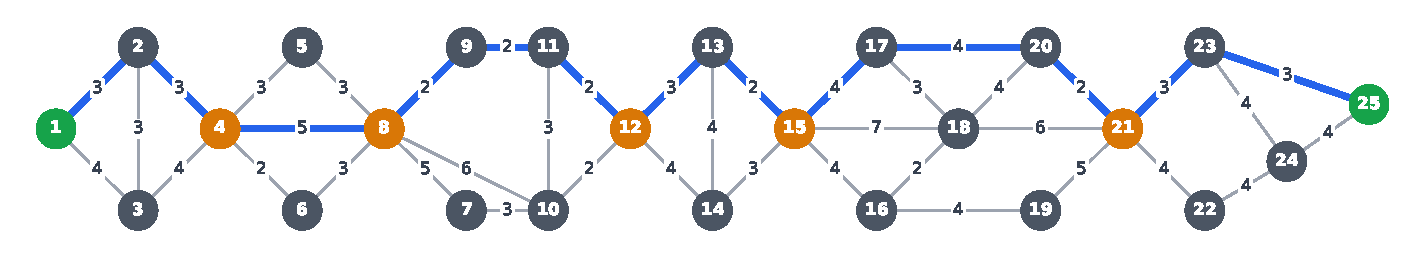
\includegraphics[width=\textwidth]{figuras/caminho_rapido.pdf}
  \caption{Rota de menor tempo (Dijkstra): 13 portas, 38 minutos.}
  \label{fig:rapido}
\end{figure}

\begin{figure}[H]
  \centering
  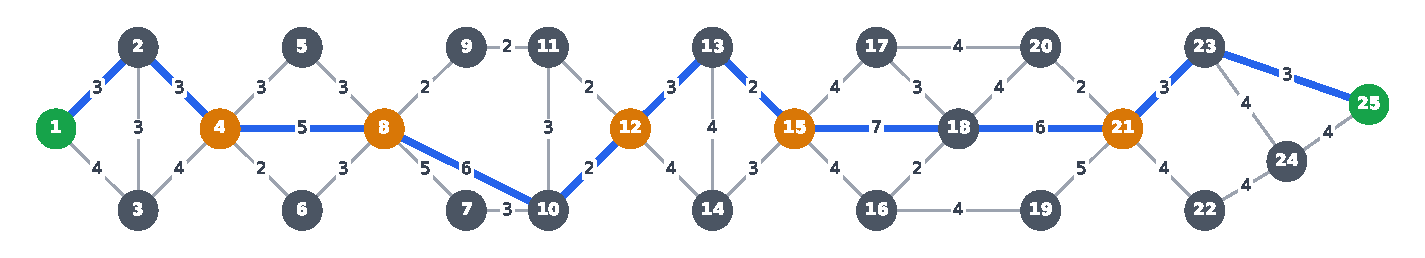
\includegraphics[width=\textwidth]{figuras/caminho_portas.pdf}
  \caption{Rota com menos portas (busca em largura): 11 portas, 43 minutos.}
  \label{fig:portas}
\end{figure}

\subsection{Imprevistos no laboratório}

Simulamos quatro situações, sempre de $v_1$ a $v_{25}$ com limite de 40 minutos,
usando os bloqueios da Definição~\ref{def:bloqueio}: fumaça em uma sala bloqueia
o vértice, e um corredor alagado fecha a aresta. A Tabela~\ref{tab:cenarios} traz
o tempo e, entre parênteses, o número de portas da rota encontrada por cada
algoritmo.

\begin{table}[H]
  \centering
  \caption{Resultados por cenário: tempo em minutos (número de portas).}
  \label{tab:cenarios}
  \begin{tabular}{lccc}
\toprule
Cenário & Menor tempo & Menos portas & Escapa? \\
\midrule
Mapa original & 38 (13) & 43 (11) & sim \\
Fumaça na $v_{17}$ & 40 (13) & 43 (11) & sim \\
Corredor $v_9$--$v_{11}$ alagado & 40 (12) & 43 (11) & sim \\
Os dois juntos & 42 (12) & 43 (11) & não \\
Sala de controle trancada & $\infty$ & $\infty$ & não \\
\bottomrule
\end{tabular}

\end{table}

As rotas de menor tempo de cada cenário são:

\begin{itemize}
\item \textbf{Mapa original:} $v_{1} \to v_{2} \to v_{4} \to v_{8} \to v_{9} \to v_{11} \to v_{12} \to v_{13} \to v_{15} \to v_{17} \to v_{20} \to v_{21} \to v_{23} \to v_{25}$.
\item \textbf{Fumaça na $v_{17}$:} $v_{1} \to v_{2} \to v_{4} \to v_{8} \to v_{9} \to v_{11} \to v_{12} \to v_{13} \to v_{15} \to v_{16} \to v_{18} \to v_{21} \to v_{23} \to v_{25}$.
\item \textbf{Corredor $v_9$--$v_{11}$ alagado:} $v_{1} \to v_{2} \to v_{4} \to v_{8} \to v_{10} \to v_{12} \to v_{13} \to v_{15} \to v_{17} \to v_{20} \to v_{21} \to v_{23} \to v_{25}$.
\item \textbf{Os dois juntos:} $v_{1} \to v_{2} \to v_{4} \to v_{8} \to v_{10} \to v_{12} \to v_{13} \to v_{15} \to v_{16} \to v_{18} \to v_{21} \to v_{23} \to v_{25}$.
\item \textbf{Sala de controle trancada:} não há caminho.
\end{itemize}


\begin{figure}[H]
  \centering
  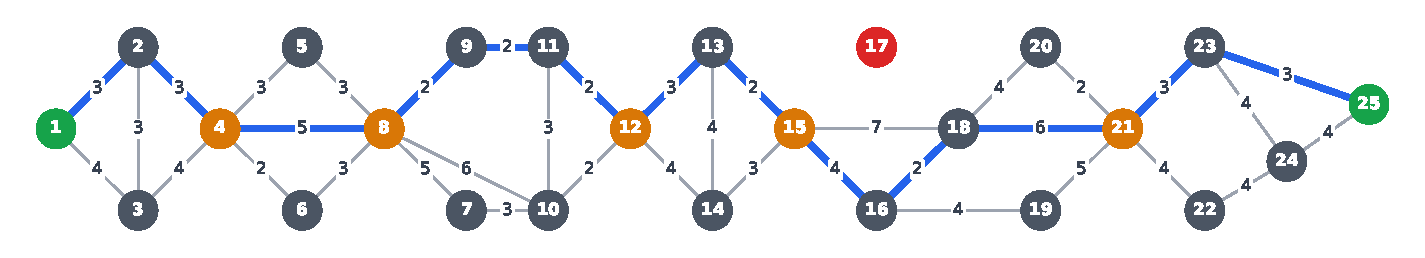
\includegraphics[width=\textwidth]{figuras/cenario_fumaca.pdf}\\[2pt]
  {\small (a) Fumaça na $v_{17}$: 40 minutos.}\\[8pt]
  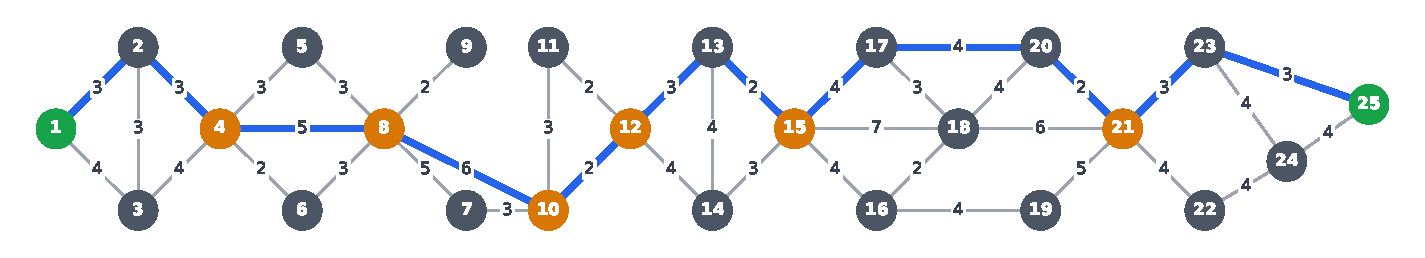
\includegraphics[width=\textwidth]{figuras/cenario_alagado.pdf}\\[2pt]
  {\small (b) Corredor $v_9$--$v_{11}$ alagado: 40 minutos. A sala $v_{10}$ passa a ser obrigatória.}
  \caption{Um imprevisto: a fuga ainda é possível, mas no limite.}
\end{figure}

\begin{figure}[H]
  \centering
  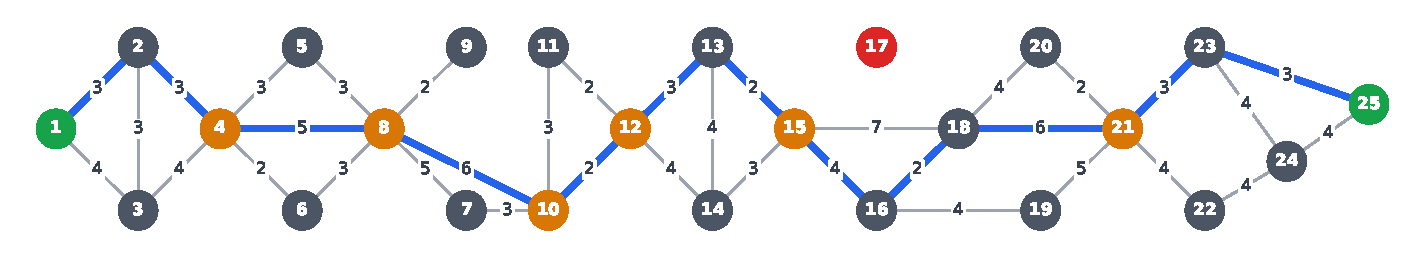
\includegraphics[width=\textwidth]{figuras/cenario_dois.pdf}\\[2pt]
  {\small (a) Os dois imprevistos juntos: 42 minutos.}\\[8pt]
  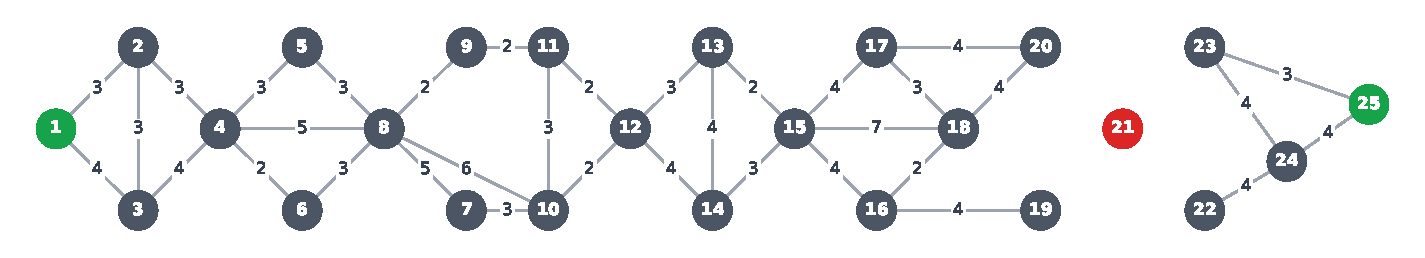
\includegraphics[width=\textwidth]{figuras/cenario_controle.pdf}\\[2pt]
  {\small (b) Sala de controle $v_{21}$ trancada: não há rota de fuga.}
  \caption{Situações em que a fuga é impossível.}
\end{figure}

Cada imprevisto sozinho custa exatamente 2 minutos e consome toda a folga, e os
dois juntos impedem a fuga. Fechar o corredor $v_9$--$v_{11}$ faz com que toda
rota passe por $v_{10}$, que se torna uma sala obrigatória: uma obstrução pode
criar novos pontos críticos. Já trancar $v_{21}$ é o caso do
Corolário~\ref{cor:bloqueio}: nenhuma mudança de tempo resolve, porque não existe
rota de fuga.

\subsection{Aplicação: evacuação em uma enchente}

A mesma modelagem se aplica à evacuação de uma cidade hipotética durante uma
enchente, em que as pessoas precisam sair do Centro e chegar a um abrigo em área
segura. Agora, os vértices são bairros e pontos de passagem, e as arestas são as
ligações entre eles: $v_{1}$ Centro, $v_{2}$ Bairro Ribeirinho, $v_{3}$ Bairro Leste, $v_{4}$ Ponte, $v_{5}$ Margem Oeste, $v_{6}$ Vila Oeste, $v_{7}$ Bairro Industrial, $v_{8}$ Vila Norte, $v_{9}$ Avenida Norte, $v_{10}$ Colina, $v_{11}$ Entroncamento, $v_{12}$ Estrada Alta, $v_{13}$ Estrada da Serra, $v_{14}$ Abrigo
. A entrada é $v_1$, a saída é
$v_{14}$ e o tempo limite é de 120 minutos. Os pesos são tempos hipotéticos, em
minutos, escolhidos para ilustrar o método.

\begin{figure}[H]
  \centering
  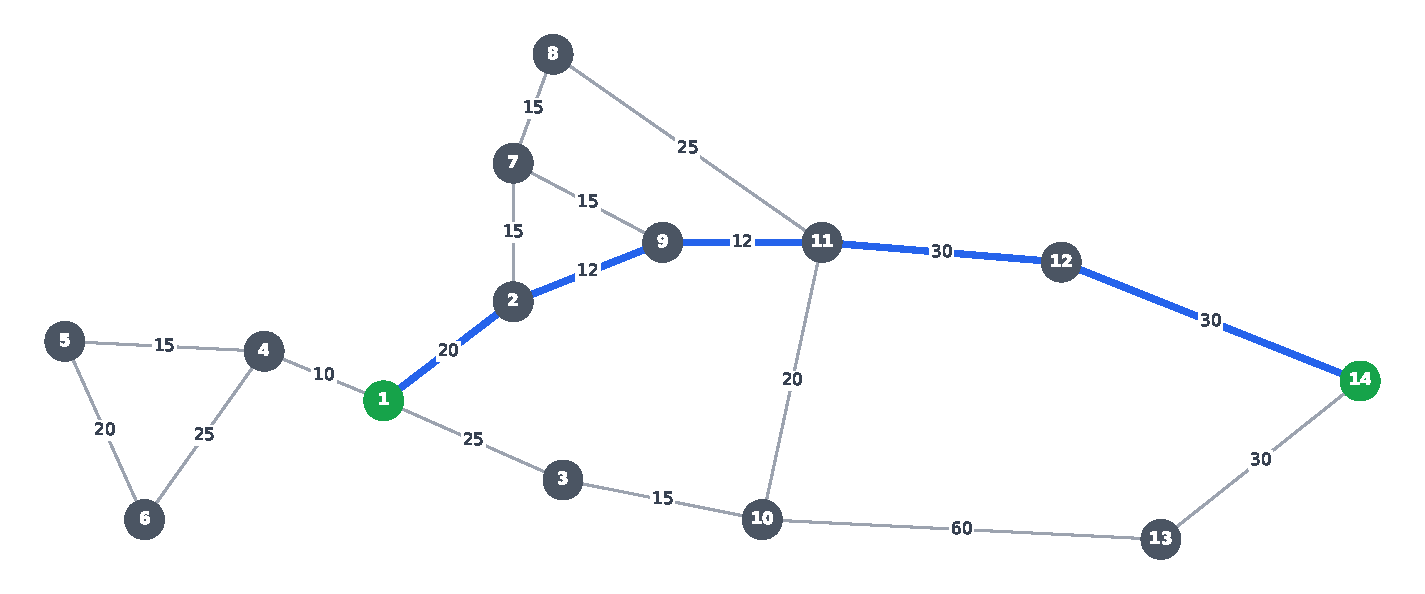
\includegraphics[width=0.75\textwidth]{figuras/enchente_0.pdf}
  \caption{Sem bloqueios: a rota de menor tempo (azul) passa pelo Bairro Ribeirinho,
  pela Avenida Norte, pelo Entroncamento e pela Estrada Alta.}
\end{figure}

\begin{table}[H]
  \centering
  \caption{Evacuação na enchente: tempo em minutos (número de ligações).}
  \label{tab:enchente}
  \begin{tabular}{lccc}
\toprule
Situação & Menor tempo & Menos ligações & Escapa? \\
\midrule
Sem bloqueios & 104 (5) & 130 (4) & sim \\
Ponte fechada ($v_4$) & 104 (5) & 130 (4) & sim \\
Bairro Ribeirinho alagado ($v_2$) & 120 (5) & 130 (4) & sim \\
Bairro alagado e estrada fechada ($v_2$; $v_{10}$--$v_{11}$) & 130 (4) & 130 (4) & não \\
Bairro e Colina bloqueados ($v_2$; $v_{10}$) & $\infty$ & $\infty$ & não \\
\bottomrule
\end{tabular}

\end{table}

\begin{figure}[H]
  \centering
  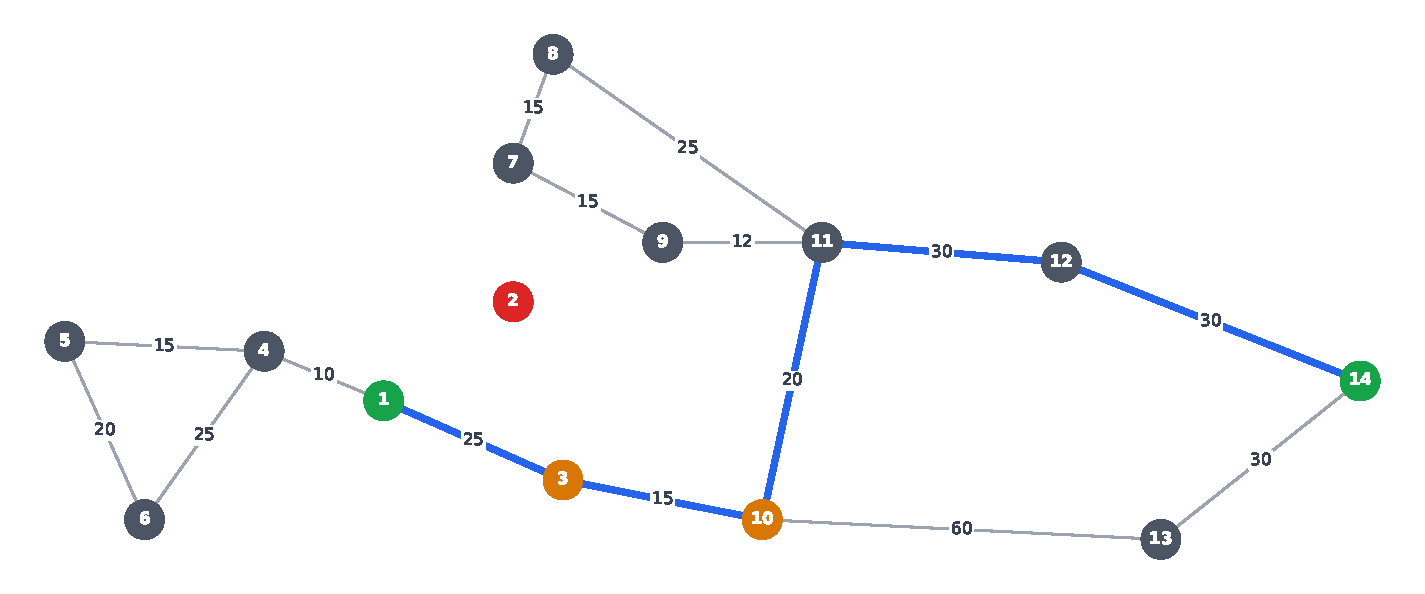
\includegraphics[width=0.75\textwidth]{figuras/enchente_2.pdf}
  \caption{Bairro Ribeirinho alagado: a rota passa pelo Bairro Leste e pela Colina,
  que se tornam obrigatórios.}
\end{figure}

Os mesmos fenômenos do escape room reaparecem: a rota com menos ligações
(130 minutos) é mais lenta que a de menor tempo (104 minutos) e não cabe no limite.
Fechar a ponte não altera a melhor rota, porque ela leva para o lado oposto ao
abrigo. Já o alagamento do Bairro Ribeirinho leva o tempo exatamente ao limite de
120 minutos e torna o Bairro Leste e a Colina obrigatórios. Se a estrada entre a
Colina e o Entroncamento também for fechada, a fuga leva 130 minutos; e, se a Colina
for bloqueada, não resta nenhuma rota.

\subsection{Implementação e simulador}

Os algoritmos foram implementados em Python sem bibliotecas de grafos; a
biblioteca NetworkX foi usada apenas nos testes automáticos, para conferir os
resultados em 200 grafos aleatórios. O grafo é guardado como lista de adjacência:
para cada vértice $v$, guardamos $N(v)$ e os pesos das arestas. O simulador,
feito com Streamlit, mostra o grafo com as rotas do Dijkstra e da busca em
largura; clicando em um vértice, a sala é bloqueada e tudo é recalculado. Também é
possível alterar pesos, fechar portas, trocar a entrada e a saída e importar uma
matriz de pesos qualquer, como a do cenário de enchente.


\section{Conclusão}\label{sec:conclusao}

Modelar o escape room como um grafo com pesos transformou o desafio da fuga em um
problema de distâncias, e os resultados demonstrados respondem a ele. A fuga é
possível: o Algoritmo de Dijkstra encontra uma rota de 38 minutos, dentro do
limite de 40. Por outro lado, a rota com menos portas, encontrada pela busca em
largura, tem 11 portas e leva 43 minutos, e as potências da matriz de adjacência
mostram que todas as 4 rotas com 11 portas levam entre 43 e 47 minutos. Minimizar
o número de passagens não é o mesmo que minimizar o tempo, e só o critério com
pesos garante a fuga.

As salas obrigatórias da história, $v_4$, $v_8$, $v_{12}$, $v_{15}$ e $v_{21}$,
são exatamente as que separam a entrada da saída, e bloquear qualquer uma delas
torna a distância infinita. As simulações mostram ainda que a folga é pequena: um
imprevisto consome os 2 minutos de margem e dois imprevistos impedem a fuga.

Por fim, a mesma lógica se aplicou a um cenário de enchente: sem bloqueios, a saída
do Centro até o abrigo leva 104 minutos; com o Bairro Ribeirinho alagado, 120 minutos,
exatamente no limite; com a estrada da Colina também fechada, 130 minutos, acima do
limite; e, com a Colina bloqueada, não existe rota. Isso confirma a ideia central do trabalho: resolvido o problema da
travessia em um escape room, o mesmo modelo e os mesmos algoritmos servem para
planejar rotas de fuga em contextos reais.

\begin{bibliografia}{9}
\bibitem{notas} Notas de aula de Matemática Discreta, FGV EMAp, 2026.
\bibitem{johnsonbaugh} R. Johnsonbaugh. \emph{Discrete Mathematics}. Pearson.
\bibitem{rangel} S. Rangel. \emph{Teoria dos Grafos}. UNESP.
\bibitem{wilson} R. J. Wilson. \emph{Introduction to Graph Theory}. Pearson.
\bibitem{dijkstra} E. W. Dijkstra. A note on two problems in connexion with
  graphs. \emph{Numerische Mathematik}, 1:269--271, 1959.
\end{bibliografia}

\section{Material de Apoio: Matrizes do grafo do \textit{escape room}\label{ap:matrizes}

\begin{table}[H]
  \centering
  \caption{Matriz de adjacência $A$ (Definição~\ref{def:adjacencia}).}
  \resizebox{\textwidth}{!}{\begin{tabular}{c|ccccccccccccccccccccccccc}
 & $v_{1}$ & $v_{2}$ & $v_{3}$ & $v_{4}$ & $v_{5}$ & $v_{6}$ & $v_{7}$ & $v_{8}$ & $v_{9}$ & $v_{10}$ & $v_{11}$ & $v_{12}$ & $v_{13}$ & $v_{14}$ & $v_{15}$ & $v_{16}$ & $v_{17}$ & $v_{18}$ & $v_{19}$ & $v_{20}$ & $v_{21}$ & $v_{22}$ & $v_{23}$ & $v_{24}$ & $v_{25}$ \\ \hline
$v_{1}$ & 0 & 1 & 1 & 0 & 0 & 0 & 0 & 0 & 0 & 0 & 0 & 0 & 0 & 0 & 0 & 0 & 0 & 0 & 0 & 0 & 0 & 0 & 0 & 0 & 0 \\
$v_{2}$ & 1 & 0 & 1 & 1 & 0 & 0 & 0 & 0 & 0 & 0 & 0 & 0 & 0 & 0 & 0 & 0 & 0 & 0 & 0 & 0 & 0 & 0 & 0 & 0 & 0 \\
$v_{3}$ & 1 & 1 & 0 & 1 & 0 & 0 & 0 & 0 & 0 & 0 & 0 & 0 & 0 & 0 & 0 & 0 & 0 & 0 & 0 & 0 & 0 & 0 & 0 & 0 & 0 \\
$v_{4}$ & 0 & 1 & 1 & 0 & 1 & 1 & 0 & 1 & 0 & 0 & 0 & 0 & 0 & 0 & 0 & 0 & 0 & 0 & 0 & 0 & 0 & 0 & 0 & 0 & 0 \\
$v_{5}$ & 0 & 0 & 0 & 1 & 0 & 0 & 0 & 1 & 0 & 0 & 0 & 0 & 0 & 0 & 0 & 0 & 0 & 0 & 0 & 0 & 0 & 0 & 0 & 0 & 0 \\
$v_{6}$ & 0 & 0 & 0 & 1 & 0 & 0 & 0 & 1 & 0 & 0 & 0 & 0 & 0 & 0 & 0 & 0 & 0 & 0 & 0 & 0 & 0 & 0 & 0 & 0 & 0 \\
$v_{7}$ & 0 & 0 & 0 & 0 & 0 & 0 & 0 & 1 & 0 & 1 & 0 & 0 & 0 & 0 & 0 & 0 & 0 & 0 & 0 & 0 & 0 & 0 & 0 & 0 & 0 \\
$v_{8}$ & 0 & 0 & 0 & 1 & 1 & 1 & 1 & 0 & 1 & 1 & 0 & 0 & 0 & 0 & 0 & 0 & 0 & 0 & 0 & 0 & 0 & 0 & 0 & 0 & 0 \\
$v_{9}$ & 0 & 0 & 0 & 0 & 0 & 0 & 0 & 1 & 0 & 0 & 1 & 0 & 0 & 0 & 0 & 0 & 0 & 0 & 0 & 0 & 0 & 0 & 0 & 0 & 0 \\
$v_{10}$ & 0 & 0 & 0 & 0 & 0 & 0 & 1 & 1 & 0 & 0 & 1 & 1 & 0 & 0 & 0 & 0 & 0 & 0 & 0 & 0 & 0 & 0 & 0 & 0 & 0 \\
$v_{11}$ & 0 & 0 & 0 & 0 & 0 & 0 & 0 & 0 & 1 & 1 & 0 & 1 & 0 & 0 & 0 & 0 & 0 & 0 & 0 & 0 & 0 & 0 & 0 & 0 & 0 \\
$v_{12}$ & 0 & 0 & 0 & 0 & 0 & 0 & 0 & 0 & 0 & 1 & 1 & 0 & 1 & 1 & 0 & 0 & 0 & 0 & 0 & 0 & 0 & 0 & 0 & 0 & 0 \\
$v_{13}$ & 0 & 0 & 0 & 0 & 0 & 0 & 0 & 0 & 0 & 0 & 0 & 1 & 0 & 1 & 1 & 0 & 0 & 0 & 0 & 0 & 0 & 0 & 0 & 0 & 0 \\
$v_{14}$ & 0 & 0 & 0 & 0 & 0 & 0 & 0 & 0 & 0 & 0 & 0 & 1 & 1 & 0 & 1 & 0 & 0 & 0 & 0 & 0 & 0 & 0 & 0 & 0 & 0 \\
$v_{15}$ & 0 & 0 & 0 & 0 & 0 & 0 & 0 & 0 & 0 & 0 & 0 & 0 & 1 & 1 & 0 & 1 & 1 & 1 & 0 & 0 & 0 & 0 & 0 & 0 & 0 \\
$v_{16}$ & 0 & 0 & 0 & 0 & 0 & 0 & 0 & 0 & 0 & 0 & 0 & 0 & 0 & 0 & 1 & 0 & 0 & 1 & 1 & 0 & 0 & 0 & 0 & 0 & 0 \\
$v_{17}$ & 0 & 0 & 0 & 0 & 0 & 0 & 0 & 0 & 0 & 0 & 0 & 0 & 0 & 0 & 1 & 0 & 0 & 1 & 0 & 1 & 0 & 0 & 0 & 0 & 0 \\
$v_{18}$ & 0 & 0 & 0 & 0 & 0 & 0 & 0 & 0 & 0 & 0 & 0 & 0 & 0 & 0 & 1 & 1 & 1 & 0 & 0 & 1 & 1 & 0 & 0 & 0 & 0 \\
$v_{19}$ & 0 & 0 & 0 & 0 & 0 & 0 & 0 & 0 & 0 & 0 & 0 & 0 & 0 & 0 & 0 & 1 & 0 & 0 & 0 & 0 & 1 & 0 & 0 & 0 & 0 \\
$v_{20}$ & 0 & 0 & 0 & 0 & 0 & 0 & 0 & 0 & 0 & 0 & 0 & 0 & 0 & 0 & 0 & 0 & 1 & 1 & 0 & 0 & 1 & 0 & 0 & 0 & 0 \\
$v_{21}$ & 0 & 0 & 0 & 0 & 0 & 0 & 0 & 0 & 0 & 0 & 0 & 0 & 0 & 0 & 0 & 0 & 0 & 1 & 1 & 1 & 0 & 1 & 1 & 0 & 0 \\
$v_{22}$ & 0 & 0 & 0 & 0 & 0 & 0 & 0 & 0 & 0 & 0 & 0 & 0 & 0 & 0 & 0 & 0 & 0 & 0 & 0 & 0 & 1 & 0 & 0 & 1 & 0 \\
$v_{23}$ & 0 & 0 & 0 & 0 & 0 & 0 & 0 & 0 & 0 & 0 & 0 & 0 & 0 & 0 & 0 & 0 & 0 & 0 & 0 & 0 & 1 & 0 & 0 & 1 & 1 \\
$v_{24}$ & 0 & 0 & 0 & 0 & 0 & 0 & 0 & 0 & 0 & 0 & 0 & 0 & 0 & 0 & 0 & 0 & 0 & 0 & 0 & 0 & 0 & 1 & 1 & 0 & 1 \\
$v_{25}$ & 0 & 0 & 0 & 0 & 0 & 0 & 0 & 0 & 0 & 0 & 0 & 0 & 0 & 0 & 0 & 0 & 0 & 0 & 0 & 0 & 0 & 0 & 1 & 1 & 0 \\
\end{tabular}
}
\end{table}

\begin{table}[H]
  \centering
  \caption{Matriz de pesos $W$, em minutos (Definição~\ref{def:matrizpesos}).}
  \resizebox{\textwidth}{!}{\begin{tabular}{c|ccccccccccccccccccccccccc}
 & $v_{1}$ & $v_{2}$ & $v_{3}$ & $v_{4}$ & $v_{5}$ & $v_{6}$ & $v_{7}$ & $v_{8}$ & $v_{9}$ & $v_{10}$ & $v_{11}$ & $v_{12}$ & $v_{13}$ & $v_{14}$ & $v_{15}$ & $v_{16}$ & $v_{17}$ & $v_{18}$ & $v_{19}$ & $v_{20}$ & $v_{21}$ & $v_{22}$ & $v_{23}$ & $v_{24}$ & $v_{25}$ \\ \hline
$v_{1}$ & 0 & 3 & 4 & $\infty$ & $\infty$ & $\infty$ & $\infty$ & $\infty$ & $\infty$ & $\infty$ & $\infty$ & $\infty$ & $\infty$ & $\infty$ & $\infty$ & $\infty$ & $\infty$ & $\infty$ & $\infty$ & $\infty$ & $\infty$ & $\infty$ & $\infty$ & $\infty$ & $\infty$ \\
$v_{2}$ & 3 & 0 & 3 & 3 & $\infty$ & $\infty$ & $\infty$ & $\infty$ & $\infty$ & $\infty$ & $\infty$ & $\infty$ & $\infty$ & $\infty$ & $\infty$ & $\infty$ & $\infty$ & $\infty$ & $\infty$ & $\infty$ & $\infty$ & $\infty$ & $\infty$ & $\infty$ & $\infty$ \\
$v_{3}$ & 4 & 3 & 0 & 4 & $\infty$ & $\infty$ & $\infty$ & $\infty$ & $\infty$ & $\infty$ & $\infty$ & $\infty$ & $\infty$ & $\infty$ & $\infty$ & $\infty$ & $\infty$ & $\infty$ & $\infty$ & $\infty$ & $\infty$ & $\infty$ & $\infty$ & $\infty$ & $\infty$ \\
$v_{4}$ & $\infty$ & 3 & 4 & 0 & 3 & 2 & $\infty$ & 5 & $\infty$ & $\infty$ & $\infty$ & $\infty$ & $\infty$ & $\infty$ & $\infty$ & $\infty$ & $\infty$ & $\infty$ & $\infty$ & $\infty$ & $\infty$ & $\infty$ & $\infty$ & $\infty$ & $\infty$ \\
$v_{5}$ & $\infty$ & $\infty$ & $\infty$ & 3 & 0 & $\infty$ & $\infty$ & 3 & $\infty$ & $\infty$ & $\infty$ & $\infty$ & $\infty$ & $\infty$ & $\infty$ & $\infty$ & $\infty$ & $\infty$ & $\infty$ & $\infty$ & $\infty$ & $\infty$ & $\infty$ & $\infty$ & $\infty$ \\
$v_{6}$ & $\infty$ & $\infty$ & $\infty$ & 2 & $\infty$ & 0 & $\infty$ & 3 & $\infty$ & $\infty$ & $\infty$ & $\infty$ & $\infty$ & $\infty$ & $\infty$ & $\infty$ & $\infty$ & $\infty$ & $\infty$ & $\infty$ & $\infty$ & $\infty$ & $\infty$ & $\infty$ & $\infty$ \\
$v_{7}$ & $\infty$ & $\infty$ & $\infty$ & $\infty$ & $\infty$ & $\infty$ & 0 & 5 & $\infty$ & 3 & $\infty$ & $\infty$ & $\infty$ & $\infty$ & $\infty$ & $\infty$ & $\infty$ & $\infty$ & $\infty$ & $\infty$ & $\infty$ & $\infty$ & $\infty$ & $\infty$ & $\infty$ \\
$v_{8}$ & $\infty$ & $\infty$ & $\infty$ & 5 & 3 & 3 & 5 & 0 & 2 & 6 & $\infty$ & $\infty$ & $\infty$ & $\infty$ & $\infty$ & $\infty$ & $\infty$ & $\infty$ & $\infty$ & $\infty$ & $\infty$ & $\infty$ & $\infty$ & $\infty$ & $\infty$ \\
$v_{9}$ & $\infty$ & $\infty$ & $\infty$ & $\infty$ & $\infty$ & $\infty$ & $\infty$ & 2 & 0 & $\infty$ & 2 & $\infty$ & $\infty$ & $\infty$ & $\infty$ & $\infty$ & $\infty$ & $\infty$ & $\infty$ & $\infty$ & $\infty$ & $\infty$ & $\infty$ & $\infty$ & $\infty$ \\
$v_{10}$ & $\infty$ & $\infty$ & $\infty$ & $\infty$ & $\infty$ & $\infty$ & 3 & 6 & $\infty$ & 0 & 3 & 2 & $\infty$ & $\infty$ & $\infty$ & $\infty$ & $\infty$ & $\infty$ & $\infty$ & $\infty$ & $\infty$ & $\infty$ & $\infty$ & $\infty$ & $\infty$ \\
$v_{11}$ & $\infty$ & $\infty$ & $\infty$ & $\infty$ & $\infty$ & $\infty$ & $\infty$ & $\infty$ & 2 & 3 & 0 & 2 & $\infty$ & $\infty$ & $\infty$ & $\infty$ & $\infty$ & $\infty$ & $\infty$ & $\infty$ & $\infty$ & $\infty$ & $\infty$ & $\infty$ & $\infty$ \\
$v_{12}$ & $\infty$ & $\infty$ & $\infty$ & $\infty$ & $\infty$ & $\infty$ & $\infty$ & $\infty$ & $\infty$ & 2 & 2 & 0 & 3 & 4 & $\infty$ & $\infty$ & $\infty$ & $\infty$ & $\infty$ & $\infty$ & $\infty$ & $\infty$ & $\infty$ & $\infty$ & $\infty$ \\
$v_{13}$ & $\infty$ & $\infty$ & $\infty$ & $\infty$ & $\infty$ & $\infty$ & $\infty$ & $\infty$ & $\infty$ & $\infty$ & $\infty$ & 3 & 0 & 4 & 2 & $\infty$ & $\infty$ & $\infty$ & $\infty$ & $\infty$ & $\infty$ & $\infty$ & $\infty$ & $\infty$ & $\infty$ \\
$v_{14}$ & $\infty$ & $\infty$ & $\infty$ & $\infty$ & $\infty$ & $\infty$ & $\infty$ & $\infty$ & $\infty$ & $\infty$ & $\infty$ & 4 & 4 & 0 & 3 & $\infty$ & $\infty$ & $\infty$ & $\infty$ & $\infty$ & $\infty$ & $\infty$ & $\infty$ & $\infty$ & $\infty$ \\
$v_{15}$ & $\infty$ & $\infty$ & $\infty$ & $\infty$ & $\infty$ & $\infty$ & $\infty$ & $\infty$ & $\infty$ & $\infty$ & $\infty$ & $\infty$ & 2 & 3 & 0 & 4 & 4 & 7 & $\infty$ & $\infty$ & $\infty$ & $\infty$ & $\infty$ & $\infty$ & $\infty$ \\
$v_{16}$ & $\infty$ & $\infty$ & $\infty$ & $\infty$ & $\infty$ & $\infty$ & $\infty$ & $\infty$ & $\infty$ & $\infty$ & $\infty$ & $\infty$ & $\infty$ & $\infty$ & 4 & 0 & $\infty$ & 2 & 4 & $\infty$ & $\infty$ & $\infty$ & $\infty$ & $\infty$ & $\infty$ \\
$v_{17}$ & $\infty$ & $\infty$ & $\infty$ & $\infty$ & $\infty$ & $\infty$ & $\infty$ & $\infty$ & $\infty$ & $\infty$ & $\infty$ & $\infty$ & $\infty$ & $\infty$ & 4 & $\infty$ & 0 & 3 & $\infty$ & 4 & $\infty$ & $\infty$ & $\infty$ & $\infty$ & $\infty$ \\
$v_{18}$ & $\infty$ & $\infty$ & $\infty$ & $\infty$ & $\infty$ & $\infty$ & $\infty$ & $\infty$ & $\infty$ & $\infty$ & $\infty$ & $\infty$ & $\infty$ & $\infty$ & 7 & 2 & 3 & 0 & $\infty$ & 4 & 6 & $\infty$ & $\infty$ & $\infty$ & $\infty$ \\
$v_{19}$ & $\infty$ & $\infty$ & $\infty$ & $\infty$ & $\infty$ & $\infty$ & $\infty$ & $\infty$ & $\infty$ & $\infty$ & $\infty$ & $\infty$ & $\infty$ & $\infty$ & $\infty$ & 4 & $\infty$ & $\infty$ & 0 & $\infty$ & 5 & $\infty$ & $\infty$ & $\infty$ & $\infty$ \\
$v_{20}$ & $\infty$ & $\infty$ & $\infty$ & $\infty$ & $\infty$ & $\infty$ & $\infty$ & $\infty$ & $\infty$ & $\infty$ & $\infty$ & $\infty$ & $\infty$ & $\infty$ & $\infty$ & $\infty$ & 4 & 4 & $\infty$ & 0 & 2 & $\infty$ & $\infty$ & $\infty$ & $\infty$ \\
$v_{21}$ & $\infty$ & $\infty$ & $\infty$ & $\infty$ & $\infty$ & $\infty$ & $\infty$ & $\infty$ & $\infty$ & $\infty$ & $\infty$ & $\infty$ & $\infty$ & $\infty$ & $\infty$ & $\infty$ & $\infty$ & 6 & 5 & 2 & 0 & 4 & 3 & $\infty$ & $\infty$ \\
$v_{22}$ & $\infty$ & $\infty$ & $\infty$ & $\infty$ & $\infty$ & $\infty$ & $\infty$ & $\infty$ & $\infty$ & $\infty$ & $\infty$ & $\infty$ & $\infty$ & $\infty$ & $\infty$ & $\infty$ & $\infty$ & $\infty$ & $\infty$ & $\infty$ & 4 & 0 & $\infty$ & 4 & $\infty$ \\
$v_{23}$ & $\infty$ & $\infty$ & $\infty$ & $\infty$ & $\infty$ & $\infty$ & $\infty$ & $\infty$ & $\infty$ & $\infty$ & $\infty$ & $\infty$ & $\infty$ & $\infty$ & $\infty$ & $\infty$ & $\infty$ & $\infty$ & $\infty$ & $\infty$ & 3 & $\infty$ & 0 & 4 & 3 \\
$v_{24}$ & $\infty$ & $\infty$ & $\infty$ & $\infty$ & $\infty$ & $\infty$ & $\infty$ & $\infty$ & $\infty$ & $\infty$ & $\infty$ & $\infty$ & $\infty$ & $\infty$ & $\infty$ & $\infty$ & $\infty$ & $\infty$ & $\infty$ & $\infty$ & $\infty$ & 4 & 4 & 0 & 4 \\
$v_{25}$ & $\infty$ & $\infty$ & $\infty$ & $\infty$ & $\infty$ & $\infty$ & $\infty$ & $\infty$ & $\infty$ & $\infty$ & $\infty$ & $\infty$ & $\infty$ & $\infty$ & $\infty$ & $\infty$ & $\infty$ & $\infty$ & $\infty$ & $\infty$ & $\infty$ & $\infty$ & 3 & 4 & 0 \\
\end{tabular}
}
\end{table}

\end{document}
